%%==================================================
%% chapter03.tex for BIT Master Thesis
%%==================================================
\chapter{基于树状区块链的出租车调度系统框架}
% 基于树状区块链的出租车调度系统的目标和研发现状简介。

本章介绍了本文所实现系统的框架和流程结构,首先是对系统的架构进行了介绍,包括区块链后台的结构功能,和车辆端和乘客端的终端功能构成;然后对系统的运行流程进行了介绍,包括乘客端的业务运行流程和车辆端的业务运行流程设计。本系统采用本章所描述的结构和流程,结合真实地理数据的矢量地图,模拟了真实地理环境,使系统的运行结果更接近真实环境下的运行情况。
\begin{figure}
  \centering
  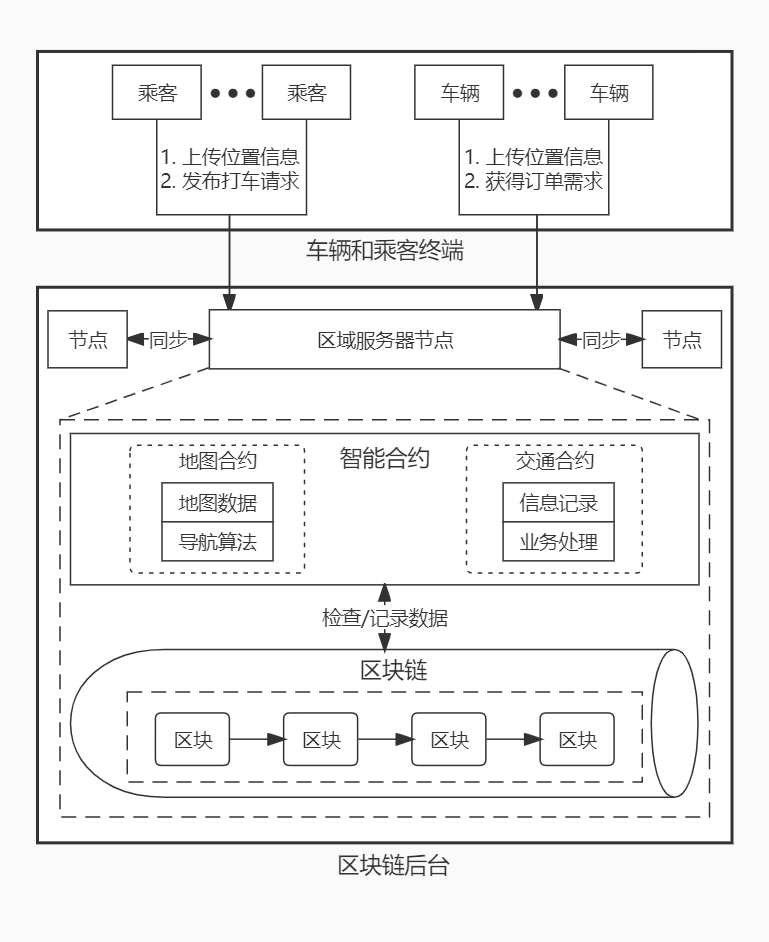
\includegraphics[width=0.75\textwidth]{figures/structure}
  \caption{出租车调度系统架构图}\label{fig:structure}
\end{figure}
% 1. 利用树状区块链
% 2. 利用GeoHash的特性
% 3. 优化A*路径规划算法
% 4. 新概念的区域调度
% 5. 实现去中心化的安全的车辆调度系统
% 6. 验证基于GeoHash地理数据和区块链研发自组网应用的可行性

\section{基于树状区块链的出租车调度系统架构设计}
% 介绍基于树状区块链的出租车调度系统的架构,由区块链后台和浏览器终端构成。
区块链后台是指按一定规律分布在城市交通系统中的路边服务节点,其上运行着自动化执行任务的智能合约。因系统后台是基于树状区块链的,故其可以通过地理信息相关的功能更好地支持整个系统。乘客和车辆的终端分别执行发单和接单的功能,以此和区块链后台一同构成完整的调度系统,如图\ref{fig:structure}所示。乘客和车辆随身运行的终端与其所属区域内的节点服务器进行交互。

\subsection{区块链上智能合约端模块}
% 介绍区块链后台模块的功能。
智能合约运行在树状区块链平台上,根据负责的功能不同分为两种合约,第一种是负责记录地理信息和执行路径规划功能的合约,本章中称其为地图合约;第二种是记录乘客和车辆的身份信息和位置信息的合约,本章中称其为交通合约。将智能合约按功能的类型分开,实现了服务端模块之间的解耦,方便了区块链系统的维护,增加了系统的稳定性和可靠性。\par

地图合约主要由地图存储模块和路径规划算法模块两个模块构成:\par
(1)地图存储模块:部署地图合约后,地图存储模块接收JS脚本上传的GeoHash矢量地图,将地图数据与不同前缀长度的GeoHash区域进行绑定,同时,将地图的三叉及多叉路口连接的道路进行存储,以方便路径规划算法在执行过程中对路口所连接道路的查找,终端可以根据GeoHash区域进行查询,向地图存储合约获取对应的矢量地图并进行展示。\par

(2)路径规划算法模块:地图合约的路径规划算法模块,是系统进行路径规划的核心部分,其接收一个起点GeoHash参数和一个终点GeoHash参数,通过改进的A*算法进行路径规划运算并返回结果。其中,一对起止点GeoHash既可以由空载车辆当时所处的位置(GeoHash表示)和乘客的上车点位置所组成,也可以由乘客的上车点位置和乘客的目的地位置所组成。路径规划算法返回的结果是一个一维数组,其元素是最短路径上所有路段的起止点。\par

除去地图存储和路径规划两个模块外,地图合约还提供了修改算法参数的接口。在以道路长度为权值的路径规划算法中,可以通过接口修改参数从而找到计算性能和准确性最优的参数。除此之外,当交通场景需求发生变化时,需要为导航算法引入不同类型的权值进行路径规划,此接口也可以方便参数的修改,以方便路径规划算法计算不同权值类型下的最短路径结果,拓展了路径规划模块的健壮性。\par

交通合约主要由信息记录模块和调度处理模块这两个模块组成:\par

(1)信息记录模块:在树状区块链上部署交通合约后,车辆和乘客登录终端,然后在智能合约的信息记录模块初始化自己的账户信息和位置信息。在初始化时乘客将自己的乘车状态设置为未乘车,车辆将自己的载客状态设置为未载客。信息记录模块同时也能改变乘客的乘车状态和车辆的载客状态,方便调度处理模块确定可调度的车辆。完成订单后,信息记录模块还会通知相关车辆乘客的支付状态,方便车辆司机判断是否可以去接下一单需求。此外,信息记录模块还给司机提供了退出系统的功能,即车辆司机需要休息或者遇到特殊情况时,可以适时退出调度系统,避免被分配到未来的需求订单。\par

(2)调度处理模块:交通合约的调度处理模块主要是将乘客和距离乘客最近的空车做匹配。乘客提交打车请求后,调度处理模块会根据乘客的位置,遍历乘客所在区域和其周围相邻的区域,寻找距离乘客最近的空车,然后将其分配给乘客。车辆在接到订单并同意后,调度处理模块会将车辆状态改为已载客。总之,调度处理模块主要完成了寻找区域内最近的空车和修改车辆和乘客状态这两个功能。


\subsection{浏览器终端模块}
% 介绍浏览器终端模块的功能。
乘客在浏览器终端通过自己的账户信息进行登录,并初始化自己所处的位置(以GeoHash表示位置),然后根据自己的位置通过web3接口从智能合约获取自己位置周边的矢量地图数据,在前端进行展示,乘客可以在渲染的地图中看到自己所处的位置。浏览器端提供了可以使乘客在智能合约记录出发点和终点的模块,然后乘客可以通过调度车辆的功能来向智能合约申请调度车辆,调度成功的车辆位置会在乘客端进行显示。在完成业务后,乘客通过web3接口进行交易确认,同时智能合约会通过监听来确认交易,在车辆确认完成订单后将车辆的状态改为未载客。\par

车辆在浏览器终端通过自己的账户信息进行登录,并初始化自己所在的位置(以GeoHash表示位置),车辆根据自己的位置通过web3接口从智能合约获取周边的矢量地图数据,在前端进行展示,可以看到自己的位置信息。如果司机需要休息或者遇到意外情况,浏览器还提供了退出按钮供车辆退出调度系统,以免接到新的需求订单。在接到乘客订单时,车主可以看到乘客的位置,判断能否顺利接到乘客,如果有困难无法接客可以选择拒绝接受此订单。在确认接受订单后,车辆可通过web3接口向智能合约申请到乘客上车点的路径规划;在确认乘客上车后,车辆可通过web3接口向智能合约申请到乘客目的地的路径规划。


\section{出租车调度系统流程设计}
% 出租车调度系统的流程设计,出租车接送客业务的企业研究现状,流程介绍。
% 出租车调度系统的流程\par
首先乘客通过浏览器终端发出乘车请求,将自己的起点和终点传到智能合约进行记录。服务器端的智能合约会记录乘客的起始点位置,通过起点的GeoHash获得乘客所在的GeoHash区域,据此进行区域调度(流程如图\ref{fig:region})来寻找最近的空车,若乘客所在的六位GeoHash区域内没有合适的车辆,则通过GeoHash邻居算法找到乘客起点相邻的8个区域,在这些区域内寻找合适的车辆,然后将最佳匹配的空车的信息通过web3回调返回给乘客端。\par

\begin{figure}
  \centering
  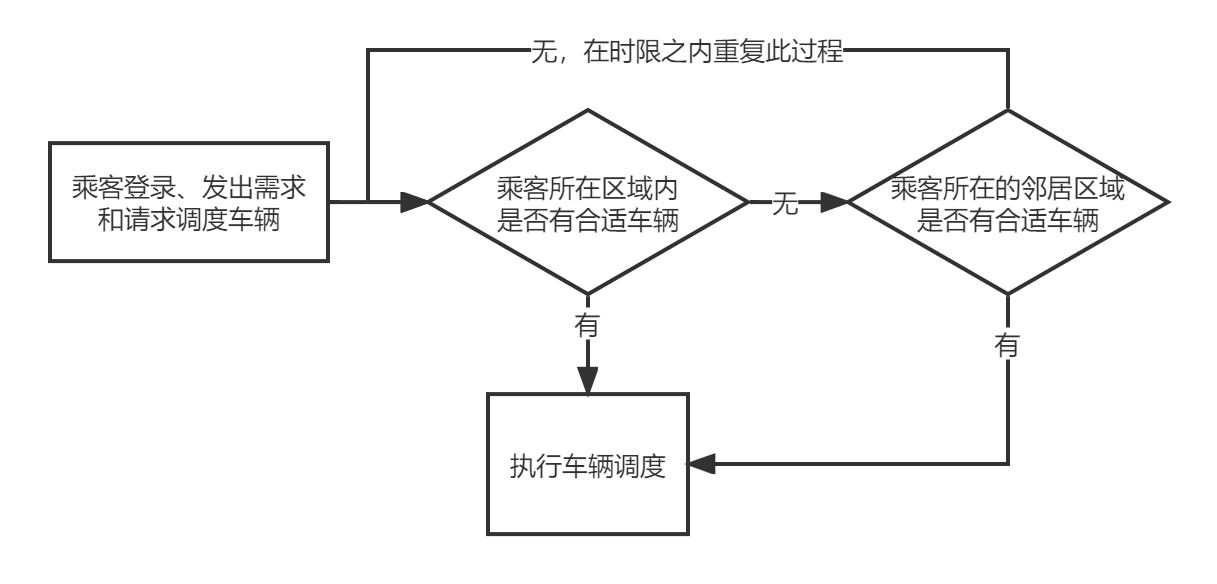
\includegraphics[width=1.0\textwidth]{figures/区域调度车辆流程}
  \caption{区域调度车辆流程}\label{fig:region}
\end{figure}

乘客端在收到车辆信息后,会通知智能合约修改车辆的载客状态和自己的乘车状态。智能合约在接收到请求后会通过assert检查该车辆的载客状态(如图\ref{fig:conflict}),即检查同一车辆是否在短时间内被分配给了不同的乘客。如果状态检查正常,则智能合约认为车辆和乘客匹配成功,顺利修改乘客的乘车状态和车辆的载客状态;如果状态检查不正确,则智能合约认为这次的车辆调度未成功,会通知乘客端重新进行呼车操作,此过程可隐式进行,方便乘客的操作。通过上述流程可以避免同一车辆被同时分配给多个乘客的错误。\par

\begin{figure}
  \centering
  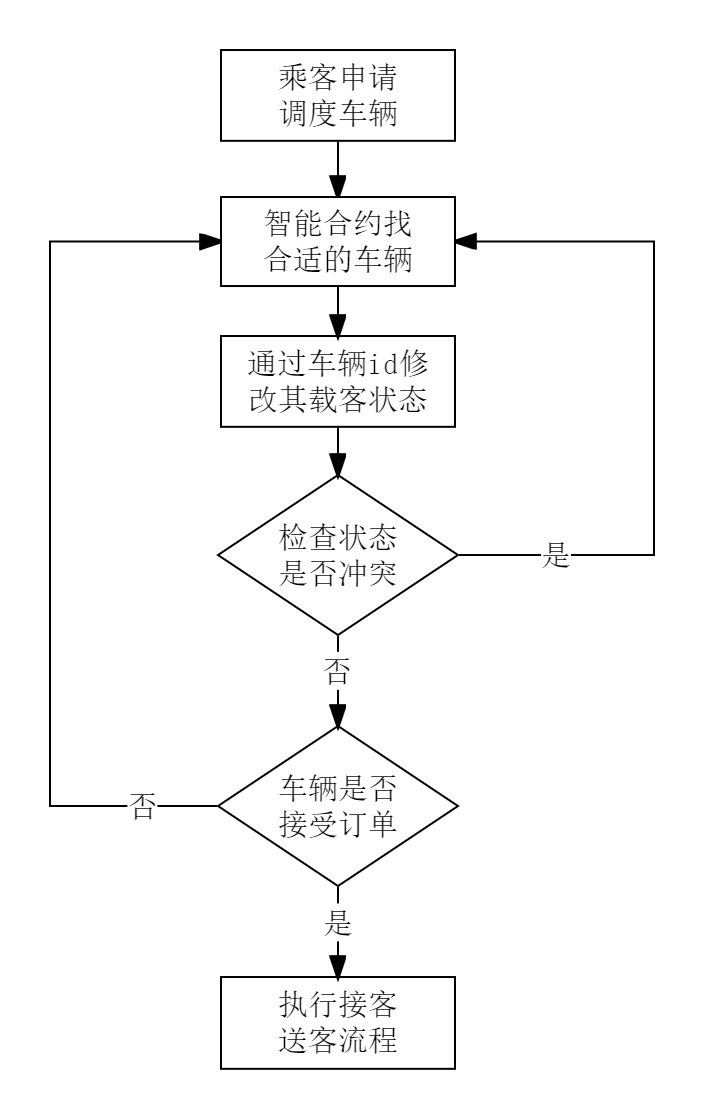
\includegraphics[width=0.55\textwidth]{figures/解决调度冲突}
  \caption{解决调度冲突流程}\label{fig:conflict}
\end{figure}

车辆和乘客匹配成功后,相关的车辆会从智能合约监听到自身的状态变化,即智能合约会把乘客的订单通知到对应的车辆。此时司机可以从终端地图上观察到乘客的位置,同时根据自己的条件和意愿选择是否去接送乘客:如果选择不接送乘客,则会将此选择反馈给智能合约,智能合约会通知乘客订单已经被取消,乘客需重新执行呼车流程,同时智能合约也不会再向原车辆提供乘客相关的信息。\par

如果车辆确认接送乘客,则如图\ref{fig:routing}所示,服务器端的智能合约会根据车辆位置和乘客的上车点执行路径规划,将路径规划的结果进行存储,并将结果通知给车辆端和乘客端,确保双方获取的路径规划结果一致,车乘双方均可在自己的终端地图观察到路径规划结果。车辆会根据路径规划结果去上车点接到乘客。乘客上车后,车辆确认接到乘客,智能合约会再次执行路径规划算法,通过乘客的上车点和终点得到最优路径,将路径规划结果进行存储,并通知车辆端和乘客端,在双方的地图上显示路径规划结果。车辆会根据最优路径将乘客送到终点。\par

\begin{figure}
  \centering
  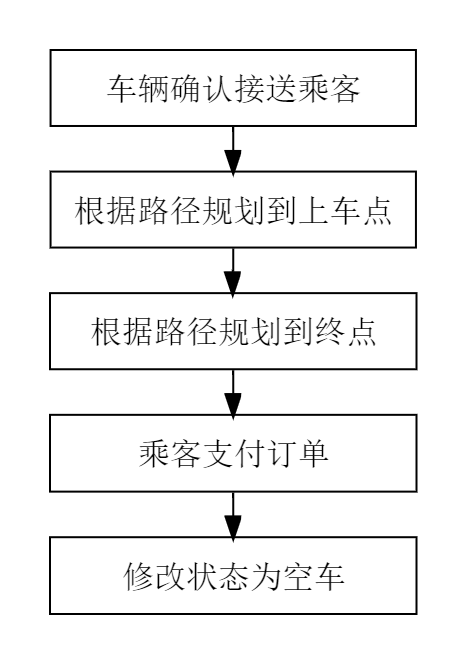
\includegraphics[width=0.35\textwidth]{figures/按导航执行业务}
  \caption{车辆执行业务流程}\label{fig:routing}
\end{figure}

车辆送乘客到达终点后,乘客执行确认到达终点的操作,表示车辆已经按路径规划结果完成任务。智能合约在接收到乘客的确认到达后,会将乘客的状态从已乘车改为未乘车,将车辆的状态从已载客改为未载客,并更新空车的位置,到此完成了一轮完整的业务流程。车辆在收到智能合约的状态改变通知后,可以根据自己当前的地理位置继续等待下一个订单任务。

% \subsection{乘客端业务流程设计}
% 介绍乘客端浏览器的业务流程。
% \subsection{出租车端业务流程设计}
% 介绍出租车端浏览器的业务流程。

\section{系统自动化运行框架的设计}
自动化运行框架基于python语法和selenium库实现,通过自动化操作浏览器运行来模拟车辆终端和乘客终端的行为(如图\ref{fig:auto})。\par

乘客端的自动化python脚本可以通过设置参数来决定打车乘客的数量。自动化脚本控制每个乘客根据自己的账户信息登录系统,然后按照各自的起止点需求和发布时间来提出打车请求。在智能合约成功记录乘客的起止点需求后,自动化脚本监听到反馈,会控制乘客端开始申请车辆调度。匹配到的车辆在确定接单后,会前来上车点接到乘客,并将乘客送到目的地。自动化脚本监听到乘客到达目的地,会执行确认和支付订单的操作,然后退出浏览器终端,视为乘客完成了一次完整业务。\par

车辆端的自动化脚本控制每辆车根据自己的账户id登录系统并初始化自己车辆的GeoHash位置,在智能合约进行记录。自动初始化完成后,车辆即可通过监听智能合约的通知来获得乘客订单并选择是否确认接受。车辆可根据即时的乘客需求来执行业务流程。此外,自动化脚本可以控制车辆的工作时长,超出工作时长后,相关车辆将会退出系统,智能合约也不再为其提供乘客订单。
\begin{figure}
  \centering
  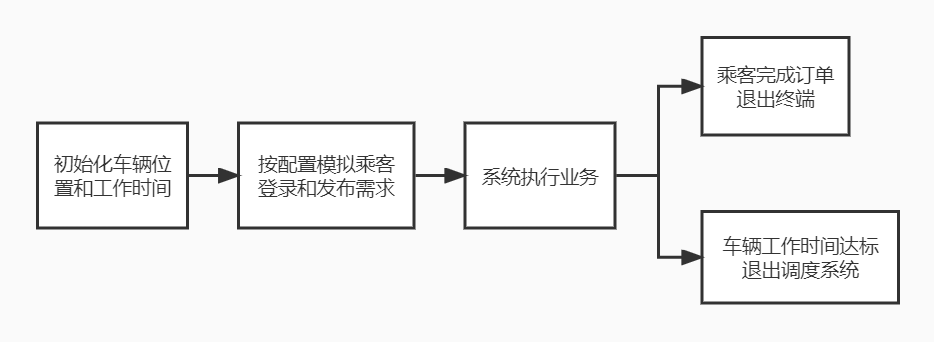
\includegraphics[width=1.0\textwidth]{figures/自动化流程}
  \caption{自动化模拟流程}\label{fig:auto}
\end{figure}

